

Adding tests to such a small solution isn't incredibly challenging. The real difficulty comes with slightly more advanced and longer programs. Over the years, I have found that as I approach over 1,000 lines of code, it slowly becomes hard to track which lines and branches are executed during tests and which aren't. After crossing 3,000 lines, it is nearly impossible. Most professional applications will have much more code than that. To deal with this problem, we can use a utility to understand which code lines are "covered" by test cases. Such code coverage tools hook up to the SUT and gather the information on the execution of each line during tests to present it in a convenient report like the one shown here:

\begin{center}
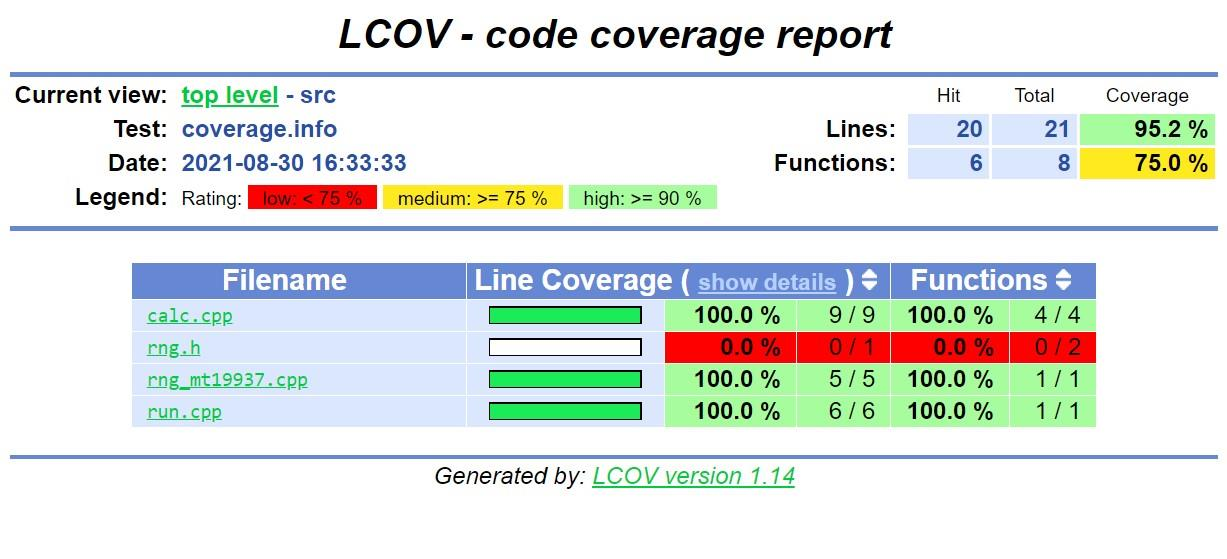
\includegraphics[width=0.8\textwidth]{content/3/chapter8/images/3.jpg}\\
Figure 8.3 ‒ Code coverage report generated by LCOV
\end{center}

These reports will show you which files are covered by tests and which aren't. More than that, you can also take a peek inside the details of each file and see exactly which lines of code are executed and how many times this occurs. In the following screenshot, the Line data column says that the Calc constructor was run 4 times, one time for each of the tests:

\begin{center}
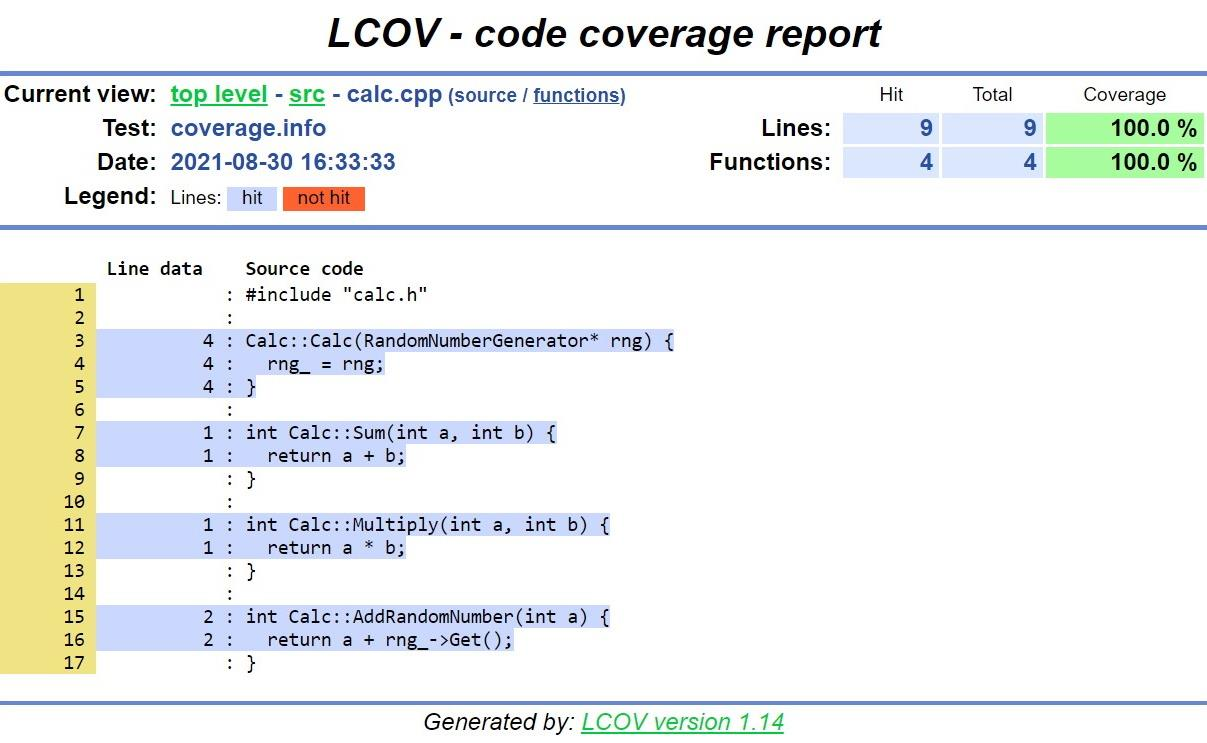
\includegraphics[width=0.8\textwidth]{content/3/chapter8/images/4.jpg}\\
Figure 8.4 ‒ Detailed view of a code coverage report
\end{center}

There are multiple ways of generating similar reports and they differ across platforms and compilers, but they generally follow the same procedure: prepare the SUT to be measured, and get the baseline, measure, and report.

The simplest tool for the job is called LCOV, and it's a graphical frontend for gcov, a coverage utility from the GNU Compiler Collection (GCC). LCOV will generate HTML coverage reports and internally use gcov to measure coverage. If you're using Clang, don't worry—Clang supports producing metrics in this format. You can get LCOV from the official repository maintained by the Linux Test Project (\url{https://github.com/linux-test-project/lcov}) or simply use a package manager. As the name suggests, it is a Linux-targeted utility. It's possible to run it on macOS, but the Windows platform is not supported. End users often don't care about test coverage, so it's usually fine to install LCOV manually in your own build environment instead of bolting it to the project.

To measure coverage, we'll need to do the following:

\begin{enumerate}
\item 
Compile in the Debug configuration with compiler flags enabling code coverage. This will generate coverage note (.gcno) files.

\item 
Link the test executable with the gcov library.

\item 
Gather coverage metrics for the baseline, without any tests being run.

\item 
Run the tests. This will create coverage data (.gcda) files.

\item 
Collect the metrics to an aggregated information file.

\item 
Generate a (.html) report.
\end{enumerate}

We should start by explaining why the code has to be compiled in the Debug configuration. The most important reason is the fact that usually, Debug configurations have disabled any optimization with a -O0 flag. CMake does this by default in the CMAKE\_CXX\_FLAGS\_DEBUG variable (despite not stating this anywhere in the documentation). Unless you decided to override this variable, your debug build should be unoptimized. This is desired to prevent any inlining and other kinds of implicit code simplification. Otherwise, it would be really hard to trace which machine instruction came from which line of source code.

In the first step, we need to instruct the compiler to add the necessary instrumentation to our SUT. The exact flag to add is compiler-specific; however, two major compilers—GCC and Clang—offer the same --coverage flag that enables coverage, producing data in a GCC-compatible gcov format.

This is how we can add the coverage instrumentation to our exemplary SUT from the previous section:

\begin{lstlisting}[style=styleCMake]
# chapter08/06-coverage/src/CMakeLists.txt

add_library(sut STATIC calc.cpp run.cpp rng_mt19937.cpp)
target_include_directories(sut PUBLIC .)
if (CMAKE_BUILD_TYPE STREQUAL Debug)
	target_compile_options(sut PRIVATE --coverage)
	target_link_options(sut PUBLIC --coverage)
	add_custom_command(TARGET sut PRE_BUILD COMMAND
						find ${CMAKE_BINARY_DIR} -type f
						-name '*.gcda' -exec rm {} +)
endif()

add_executable(bootstrap bootstrap.cpp)
target_link_libraries(bootstrap PRIVATE sut)
\end{lstlisting}

Let's break this down step by step, as follows:

\begin{enumerate}
\item 
Ensure that we're running in the Debug configuration with the if(STREQUAL) command. Remember that you won't be able to get any coverage unless you run cmake with the -DCMAKE\_BUILD\_TYPE=Debug option.

\item 
Add -{}-coverage to the PRIVATE compile options for all object files that are part of the sut library.

\item 
Add -{}-coverage to the PUBLIC linker options: both GCC and Clang interpret this as a request to link the gcov (or compatible) library with all targets that depend on sut (due to propagated properties).

\item 
The add\_custom\_command() command is introduced to clean any stale .gcda files. Reasons to add this command are discussed in detail in the Avoiding the SEGFAULT gotcha section.
\end{enumerate}

This is enough to produce code coverage. If you're using an IDE such as Clion, you'll be able to run your unit tests with coverage and get the results in a built-in report view. However, this won't work in any automated pipeline that might be run in your CI/CD. To get reports, we'll need to generate them ourselves with LCOV.

For this purpose, it's best to define a new target called coverage. To keep things clean, we'll define a separate function, AddCoverage, in another file to be used in the test listfile, as follows:

\begin{lstlisting}[style=styleCMake]
# chapter08/06-coverage/cmake/Coverage.cmake

function(AddCoverage target)
	find_program(LCOV_PATH lcov REQUIRED)
	find_program(GENHTML_PATH genhtml REQUIRED)
	
	add_custom_target(coverage
		COMMENT "Running coverage for ${target}..."
		COMMAND ${LCOV_PATH} -d . --zerocounters
		COMMAND $<TARGET_FILE:${target}>
		COMMAND ${LCOV_PATH} -d . --capture -o coverage.info
		COMMAND ${LCOV_PATH} -r coverage.info '/usr/include/*'COMMAND ${GENHTML_PATH} -o coverage filtered.info
			--legend
		COMMAND rm -rf coverage.info filtered.info
		WORKING_DIRECTORY ${CMAKE_BINARY_DIR}
		)
endfunction()
\end{lstlisting}

In the preceding snippet, we first detect the paths for lcov and genhtml (two command-line tools from the LCOV package). The REQUIRED keyword instructs CMake to throw an error when they're not found. Next, we add a custom coverage target with the following steps:

\begin{enumerate}
\item 
Clear the counters from any previous runs.

\item 
Run the target executable (using generator expressions to get its path). \$<TARGET\_FILE:target> is an exceptional generator expression, and it will implicitly add a dependency on target in this case, causing it to be built before executing all commands. We'll provide target as an argument to this function.

\item 
Remove (-r) unwanted coverage data on system headers ('/usr/include/*') and output to another file (-o filtered.info).

\item 
Generate an HTML report in the coverage directory, and add a -{}-legend color.

\item 
Remove temporary .info files.

\item 
Specifying the WORKING\_DIRECTORY keyword sets binary tree as working directory for all commands.
\end{enumerate}

These are the general steps for both GCC and Clang, but it's important to know that the gcov tool's version has to match the version of the compiler. In other words, you can't use GCC's gcov tool for Clang-compiled code. To point lcov to Clang's gcov tool, we can use the -{}-gcov-tool argument. The only problem here is that it has to be a single executable. To deal with that, we can provide a simple wrapper script (remember to mark it as an executable with chmod +x), as follows:

\begin{lstlisting}[style=stylePython]
# cmake/gcov-llvm-wrapper.sh

#!/bin/bash
exec llvm-cov gcov "$@"
\end{lstlisting}

All of our calls to \$\{LCOV\_PATH\} in the previous function should receive the following additional flag:

\begin{lstlisting}[style=stylePython]
--gcov-tool ${CMAKE_SOURCE_DIR}/cmake/gcov-llvm-wrapper.sh
\end{lstlisting}

Make sure that this function is available for inclusion in the test listfile. We can do this by extending the include search path in the main listfile, as follows:

\begin{lstlisting}[style=styleCMake]
# chapter08/06-coverage/CMakeLists.txt

cmake_minimum_required(VERSION 3.20.0)
project(Coverage CXX)
enable_testing()
list(APPEND CMAKE_MODULE_PATH "${CMAKE_SOURCE_DIR}/cmake")
add_subdirectory(src bin)
add_subdirectory(test)
\end{lstlisting}

This small line allows us to include all .cmake files from the cmake directory in our project. We can now use Coverage.cmake in the test listfile, like so:

\begin{lstlisting}[style=styleCMake]
# chapter08/06-coverage/test/CMakeLists.txt (fragment)

# ... skipped unit_tests target declaration for brevity

include(Coverage)
AddCoverage(unit_tests)

include(GoogleTest)
gtest_discover_tests(unit_tests)
\end{lstlisting}

To build this target, use the following commands (notice that first command ends with a DCMAKE\_BUILD\_TYPE=Debug build type selection):

\begin{tcblisting}{commandshell={}}
# cmake -B <binary_tree> -S <source_tree>
    -DCMAKE_BUILD_TYPE=Debug
# cmake --build <binary_tree> -t coverage
\end{tcblisting}

After executing all of the mentioned steps, you will see a short summary like this:

\begin{tcblisting}{commandshell={}}
Writing directory view page.
Overall coverage rate:
  lines......: 95.2% (20 of 21 lines)
  functions..: 75.0% (6 of 8 functions)
[100%] Built target coverage
\end{tcblisting}

Next, open the coverage/index.html file in your browser and enjoy the reports! There's only one small issue though…


\subsubsubsection{8.6.1\hspace{0.2cm}Avoiding the SEGFAULT gotcha}


We may get ourselves into trouble when we start editing sources in such a solution. This is because the coverage information is split into two parts, as follows:

\begin{itemize}
\item 
gcno files, or GNU Coverage Notes, generated during the compilation of the SUT

\item 
gcda files, or GNU Coverage Data, generated and updated during test runs
\end{itemize}

The "update" functionality is a potential source of segmentation faults. After we run our tests initially, we're left with a bunch of gcda files that don't get removed at any point. If we make some changes to the source code and recompile the object files, new gcno files will be created. However, there's no wipe step—the old gcda files still follow the stale source. When we execute the unit\_tests binary (it happens in the gtest\_discover\_tests macro), the coverage information files won't match, and we'll receive a SEGFAULT (segmentation fault) error.

To avoid this problem, we should erase any stale gcda files. Since our sut instance is a STATIC library, we can hook the add\_custom\_command(TARGET) command to building events. The clean will be executed before the rebuild starts.

Find links to more information in the Further reading section.























































